\documentclass[11pt,a4paper]{article}
\usepackage[utf8]{inputenc}
\usepackage[german]{babel}
\usepackage{amsmath}
\usepackage{amsfonts}
\usepackage{subfig}
\usepackage{amssymb}
\usepackage{siunitx,physics}
\usepackage{mathtools}
\usepackage{graphicx}
%\usepackage{Here}
\usepackage[version=4]{mhchem}
\usepackage{url}
\usepackage{setspace}
\usepackage[left=2.5cm,right=2.5cm,top=2.5cm,bottom=2cm]{geometry}
[biblography=totocnumbered]
\usepackage{fancyhdr}
\usepackage{scrextend}
\usepackage{hyperref}
\pagenumbering{gobble}

\makeatletter
\newcommand\bigcdot{\mathpalette\bigcdot@{.5}}
\newcommand\bigcdot@[2]{\mathbin{\vcenter{\hbox{\scalebox{#2}{$\m@th#1\bullet$}}}}}
\makeatother

\makeatletter
%\renewcommand*\bib@heading{%
%  \subsection*{}%
%  \@mkboth{\refname}{\refname}}
%\makeatother
\numberwithin{equation}{section}
\numberwithin{figure}{section}

\renewcommand{\labelitemii}{\labelitemfont$\vartriangleright$}
\begin{document}\\
\begin{addmargin}[25pt]{0pt}
Bei einem überwiegend duktilem Bruch kommt es im Bereich der plastischen Verformung zu Einschnürung bis der Querschnitt punktförmig ist, ersst an diesem Punkt bricht das Material. Reißt man ein duktiles Material an einer Stelle ein so verlängert sich dieser Riss nur wenn man die einwirkende Spannung erhöht, diese Art von Riss nennt man stabilen Riss. Ein mäßig duktiler Bruch hat keine extreme Einschnürung, bei ihm kommt es lediglich zu einer geringen Einschnürung bevor kleine Hohlräume gebildet werden die mit steigender Spannung immer größer werden und schließlich einen elliptischen Riss verursachen. Das andere Extrem zum duktilen Bruch ist der Sprödbruch, bei diesem kommt es zu keiner Einschnürung und es entsteht ein Riss senkrecht zur Zugrichtung mit einer flachen Bruchkante. Die 3 Arten des Bruchs sind in Abbildung \ref{fig:Brucharten} dargestellt.\\
\begin{figure}[h]
    \centering
    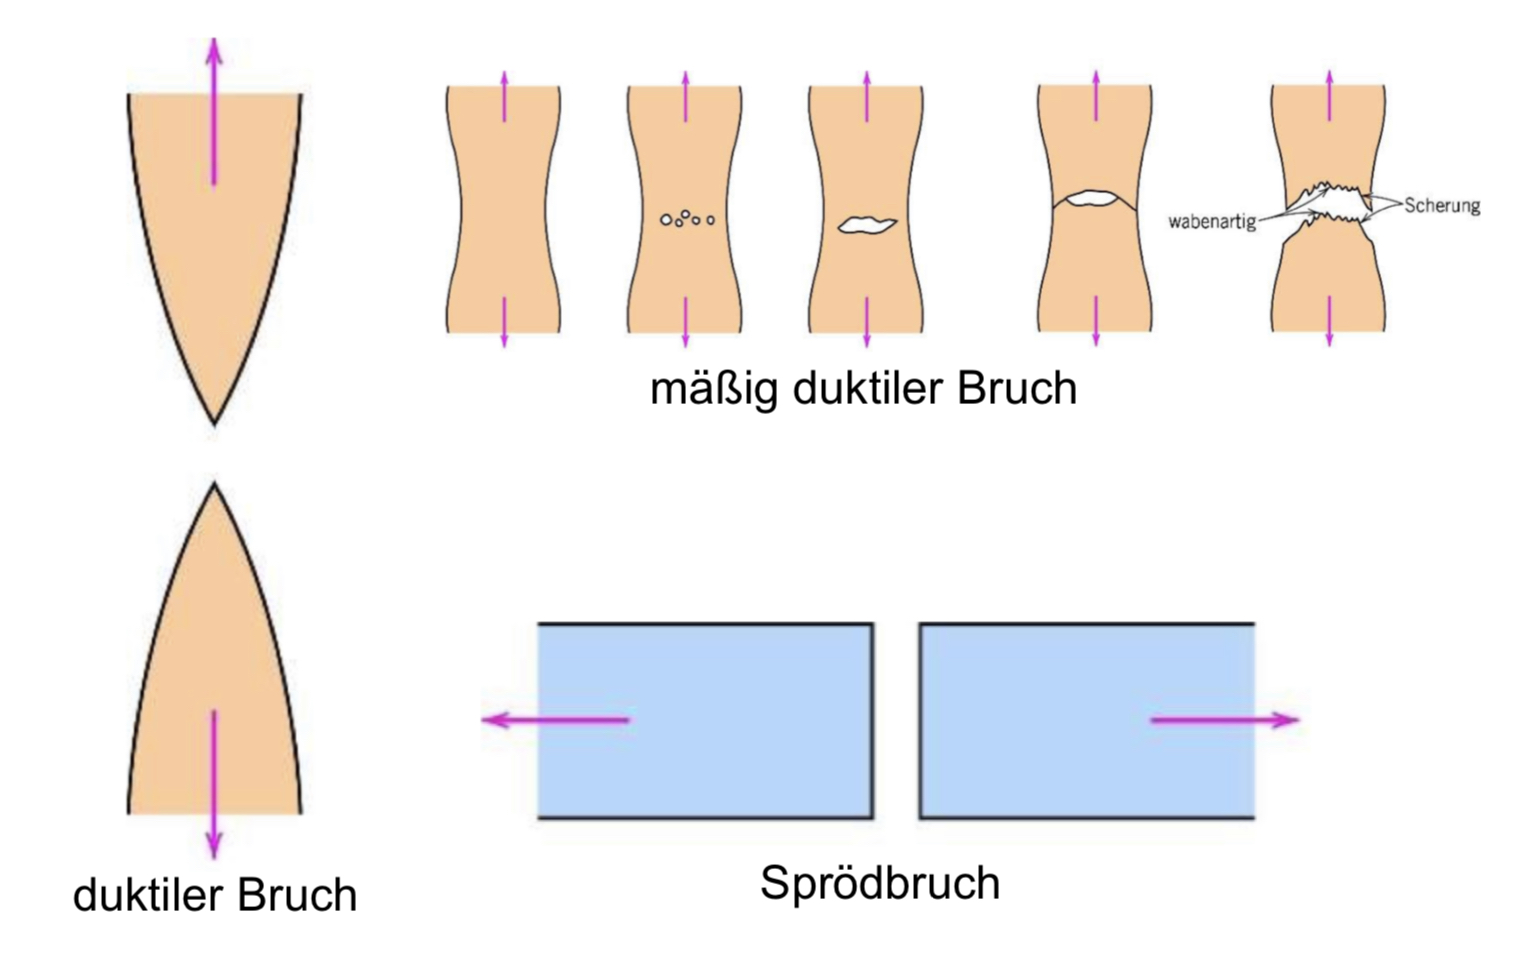
\includegraphics[width = 0.8\textwidth]{images/Materialwissenschaften/Brucharten.jpeg}
    \caption{Visualisierung der 3 Arten des Bruchs, links sieht man den duktilen Bruch, rechts oben den mäßig duktilen Bruch und rechts unten den Sprödbruch.}
    \label{fig:Brucharten}
\end{figure}
\end{addmargin}

\end{document}